\documentclass[11pt]{article}
\usepackage{colacl}
\usepackage[pdftex]{graphicx} 
\usepackage{booktabs}
\usepackage{tabularx}
\usepackage{pgfplots}
\usepackage{caption}
\usepackage{pgfplots}
\usepackage{rotating}
\usepackage{tikz}
\usepackage{float}
\usepackage[margin=1in]{geometry}
\usetikzlibrary{shapes.geometric, arrows}
\sloppy

\captionsetup[figure]{
    labelsep=period,
    justification=centering
}

\tikzstyle{startstop} = [rectangle, rounded corners, minimum width=3cm, minimum height=1cm, text centered, draw=black, fill=red!30]
\tikzstyle{io} = [trapezium, trapezium left angle=70, trapezium right angle=110, minimum width=3cm, minimum height=1cm, text centered, draw=black, fill=blue!30]
\tikzstyle{process} = [rectangle, minimum width=3cm, minimum height=1cm, text centered, draw=black, fill=orange!30]
\tikzstyle{arrow} = [thick,->,>=stealth]

\title{Exploring the impact of machine learning algorithms with unlabelled data}
\author
{Anonymous}



\begin{document}
\maketitle


%\begin{abstract}
%This is a \LaTeX\ sample for your paper.
%You shouldn't plan to include an abstract for a paper of this length.
%\end{abstract}

\section{Introduction}
Predicting salary based on job descriptions is a challenging task in the field of natural language processing and machine learning.
In the current digital age, many recruiters seek to find suitable candidates through multiple channels 
— e.g., online job portals, professional networks 
— as well as traditional avenues, such as word of mouth and mass media \cite{Primary-Organizational-Recruitment-Sources}.

The dataset is derived from the large dataset called \textit{mycareersfuture} \cite{bhola-etal-2020-retrieving}.
The dataset has a total of 17377 data, consisting of 13902 train data, 1738 validation data, and 1737 test data. 
The dataset is shown in the table \ref{tab:dataset_info}:


\begin{table}[h]
    \centering
    \caption{Dataset Information}
    \begin{tabular}{lrrr}
        \toprule
        Data Type      & Labeled & Unlabeled & Total \\
        \midrule
        Train          & 8000    & 5902      & 13902 \\
        Validation     & 1738    & -         & 1738  \\
        Test           & -       & 1737      & 1737  \\
        \midrule
        Total          & 9738    & 7639      & 17377 \\
        \bottomrule
    \end{tabular}
    \label{tab:dataset_info}
\end{table}

The distribution of salary bin is shown in the figure \ref{fig:dataset_output}.
We observe that the salary bin distribution exhibits an uneven and imbalanced pattern,
which may potentially affect the performance of the machine learning algorithms.


To answer the question "Does Unlabelled data improve Job salary prediction?", 
We will analyse and compare the performance of different machine learning algorithms for this dataset (labelled and unlabelled data) 
and finally explore whether unlabelled data can be effectively combined to increase the performance of the model.

\begin{figure}[t]
    \centering
    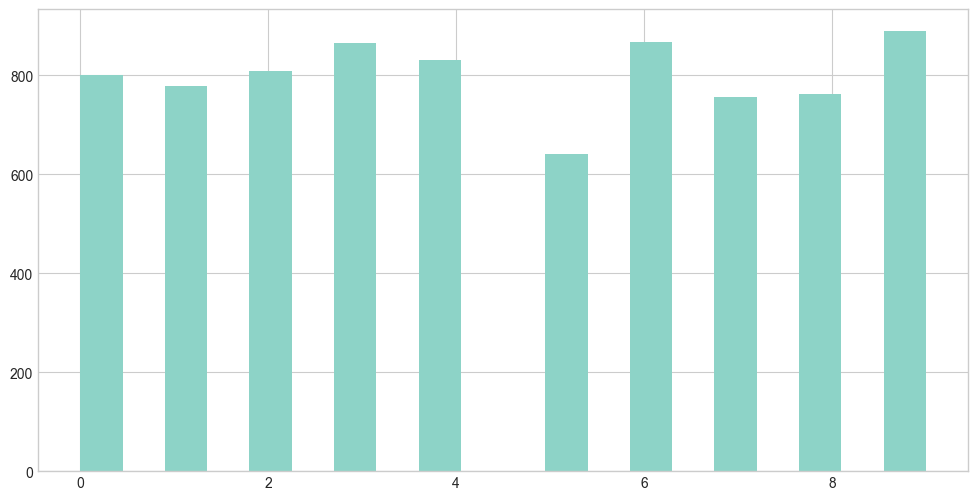
\includegraphics[width=0.5\textwidth]{dataset_output.png}
    \caption{Salary Bin Distribution}
    \label{fig:dataset_output}
\end{figure}

\section{Literature review}


\section{Methods}


In this study, we adopt two feature representations from the raw job descriptions.

\begin{itemize}
    \item \textbf{TF-IDF}: We compute the TF-IDF vectors for job descriptions using the method proposed by \cite{manning2008introduction}. This method captures the importance of terms within a document and across the entire corpus.
    \item \textbf{Embedding}: We adopt the pretrained Sentence Transformer model \cite{reimers-gurevych-2019-sentence} to obtain word embeddings for the job descriptions. These embeddings provide semantic representation for the text data.
\end{itemize}


Through these two features, we explore three different machine learning algorithms paradigms: Supervised learning, Unsupervised learning and Semi-supervised learning.

To find the parameters which can lead the highest performance of the machine learning algorithms, we consider to use some search strategies.
Due to a high dimentions of the features, we adopt Grid search here because Grid search can suffer from high dimensional spaces \cite{liashchynskyi2019grid}.

We train the models between TFIDF and Embedding features, but we will only choose TFIDF features to analyse the results and evaluate the models.
To evaluate classifiers, we use the $F_1$ score that combines recall and precision in the following way: \cite{TAN2006290}

\begin{equation}
    precision = \frac{TP}{TP + FP}
\end{equation}

\begin{equation}
    recall = \frac{TP}{TP + FN}
\end{equation}

\begin{equation}
    F_1 = 2 \times \frac{precision \times recall}{precision + recall}
\end{equation}





% In the experiment, we decided to use salary bin as our target labels.
% To predict the salary bin, we will adopt the classification machine learning algorithms.
% We split our experiment into three parts: supervised learning, unsupervised learning, and semi-supervised learning.




\subsection{Supervised learning}
In the supervised learning part, we adopt 9 different machine learning algorithms to predict the salary bin.


\subsubsection{KNN Classifier}
We decide to use k-Nearest-Neighbours (kNN) as our baseline model, because the k-Nearest-Neighbours is a simple but effective method for classification \cite{10.1007/978-3-540-39964-3_62}.
To ensure what weights and p value in KNN classifier lead to a better performance, We set k value in the range of 1 to 11,
and weight options are uniform and distance,
p value is 1 and 2 (represent manhattan distance and euclidean distance).


Using Grid search, we find that in TF-IDF, using kNN algorithm's best accuracy is 18.77\% with parameters (k = 3, p = 2, weights = "distance").
In Embedding, using kNN algorithm's best accuracy is 23.95 \% with parameters (k = 3, p = 2, weights = "distance").


\begin{figure}[b]
    \centering
    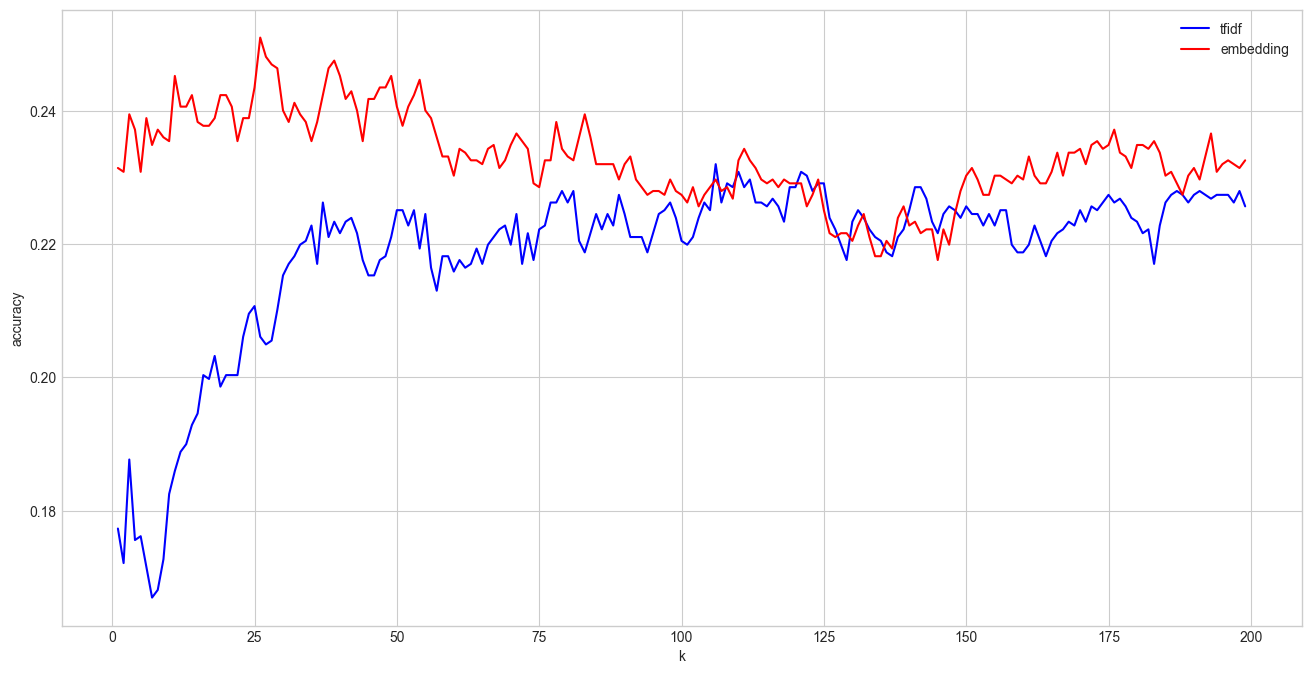
\includegraphics[width=0.5\textwidth]{knn_output.png}
    \caption{KNN Classifier}
    \label{fig:knn}
\end{figure}

In the experiment, we found that K is the most important factor in kNN algorithm. 
So we keep increasing k's value to 200.
And set p equal to 2 and weight is "distance". 
The output is shown in figure \ref{fig:knn}.


From the results, we can when the k value is 106, the accuracy for tfidf is 23.20\% which is the best accuracy for tfidf.
For embedding data, the best accuracy is 25.1\% when k is 26.


\subsubsection{Decision Tree Classifier}

Decision
It focuses on generating classification rules displayed as decision trees that is deduced or concluded from a group of disorder and irregular instances. \cite{dt_8718711}

\subsubsection{Naive Bayes Classifier}


\subsubsection{Other Classifier}


\subsection{Unsupervised learning}


\subsection{Semi-supervised learning}
we will use the architecture shown in figure \ref{fig:Self-trained} to train the model.

\begin{figure}[t]
    \centering
    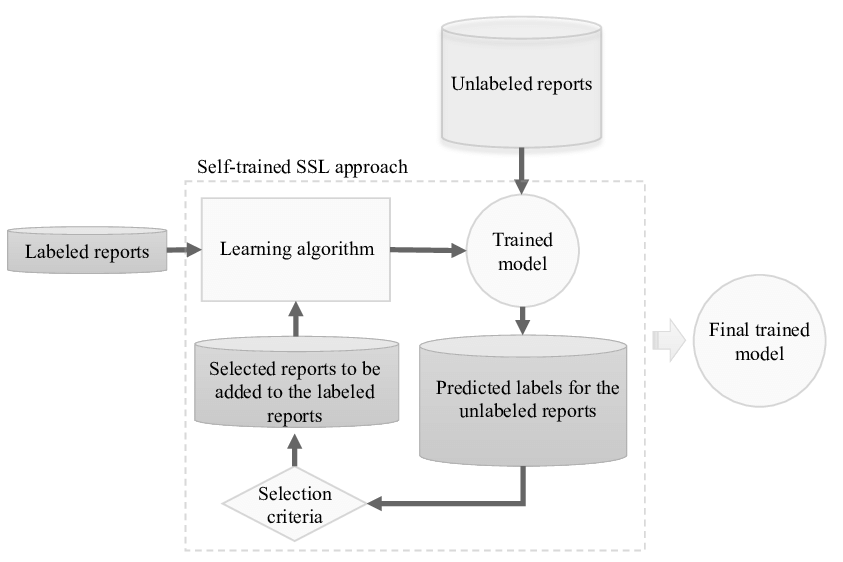
\includegraphics[width=0.5\textwidth]{Self-trained-semi-supervised-learning-architecture.png}
    \caption{Self-trained semi-supervised learning architecture \cite{Self-trained-semi-supervised-learning}}
    \label{fig:Self-trained}
\end{figure}




\section{Results}

\section{Discussion / Critical Analysis}

\section{Conclusions}





\begin{figure*}
    \centering
    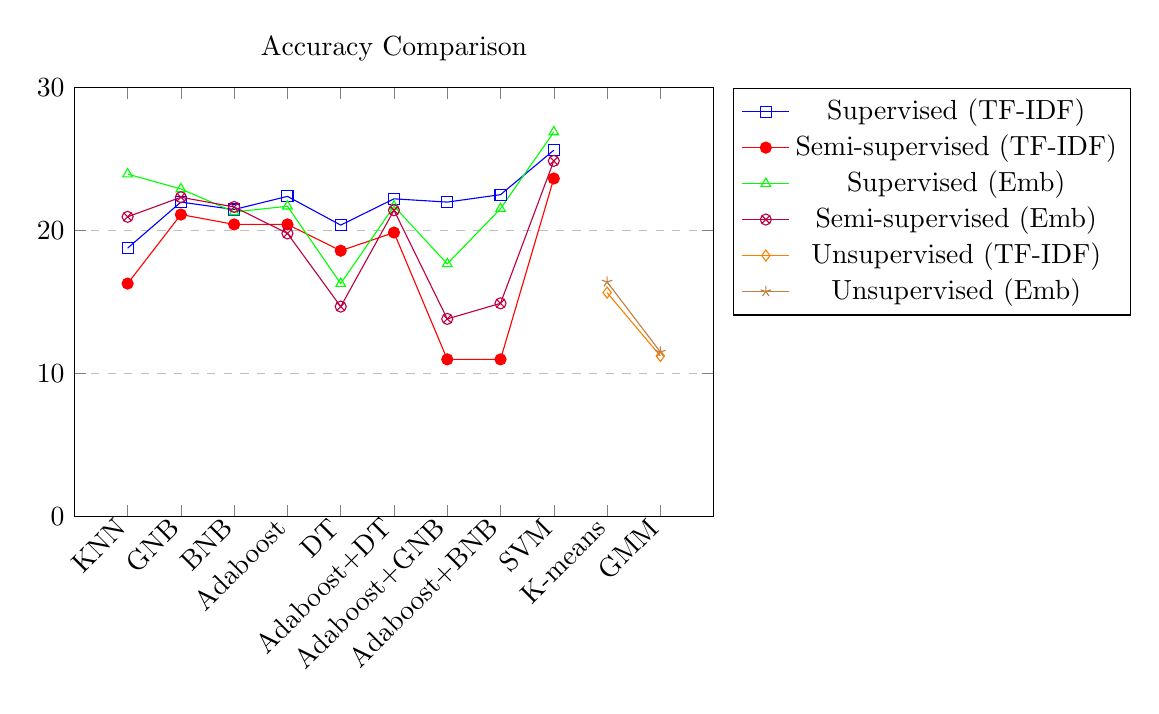
\begin{tikzpicture}
        \begin{axis}[
            title={Accuracy Comparison},
            % xlabel={Models},
            % ylabel={Accuracy},
            xmin=0, xmax=12,
            ymin=0, ymax=30,
            xtick={1, 2, 3, 4, 5, 6, 7, 8, 9, 10, 11, 12},
            xticklabels={
                KNN, GNB, BNB, Adaboost, DT, Adaboost+DT, Adaboost+GNB, Adaboost+BNB, SVM, K-means, GMM},
            xticklabel style={rotate=45, anchor=east},
            legend pos=outer north east,
            ymajorgrids=true,
            grid style=dashed,
            width=0.8\textwidth,
            height=200,
        ]
    
        % Labeled data (TFIDF)
        \addplot[
            color=blue,
            mark=square,
        ]
        coordinates {
            (1,18.77) (2,21.99) (3,21.47) (4,22.39) (5,20.38) (6,22.22) (7,21.99) (8,22.51) (9,25.62)
        };
        \addlegendentry{Supervised (TF-IDF)}
        
        % Unlabeled data (TFIDF)
        \addplot[
            color=red,
            mark=*,
        ]
        coordinates {
            (1,16.29) (2,21.12) (3,20.43) (4,20.43) (5,18.59) (6,19.86) (7,10.99) (8,10.99) (9,23.64)
        };
        \addlegendentry{Semi-supervised (TF-IDF)}
        
        % Labeled data (Embedding)
        \addplot[
            color=green,
            mark=triangle,
        ]
        coordinates {
            (1,23.95) (2,22.91) (3,21.3) (4,21.7) (5,16.29) (6,21.7) (7,17.67) (8,21.53) (9,26.89)
        };
        \addlegendentry{Supervised (Emb)}
    
        % Unlabeled data (Embedding) - Semi-supervised
        \addplot[
            color=purple,
            mark=otimes,
        ]
        coordinates {
            (1,20.96) (2,22.33) (3,21.65) (4,19.8) (5,14.68) (6,21.42) (7,13.82) (8,14.91) (9,24.87)
        };
        \addlegendentry{Semi-supervised (Emb)}
        
        % Unlabeled data (Embedding)
        \addplot[
            color=orange,
            mark=diamond,
        ]
        coordinates {
            (10,15.66) (11,11.23)
        };
        \addlegendentry{Unsupervised (TF-IDF)}

        \addplot[
            color=brown,
            mark=star,
        ]
        coordinates {
            (10,16.41) (11,11.51)
        };
        \addlegendentry{Unsupervised (Emb)}
        
        \end{axis}
    \end{tikzpicture}
\end{figure*}



\begin{table*}
    \begin{center}
        \captionof{table}{Accuracy Comparison} \label{tab:title} 
        \begin{tabularx}{\textwidth}{@{}l *{7}{>{\centering\arraybackslash}X} @{}}
        \toprule
        Model & \multicolumn{2}{c}{TFIDF} & \multicolumn{2}{c}{Embedding}\\
        \cmidrule(lr){2-3} \cmidrule(lr){4-5}
        & Labaled data & Unlabeled data & Labaled data & Unlabaled data \\
        \midrule
        
        	KNN & 18.77 & 16.29 & 23.95 & 20.96 \\
        	GNB & 21.99 & 21.12 & 22.91 & 22.33 \\
        	BNB  & 21.47 & 20.43 & 21.3 & 21.65 \\
        	Adaboost & 22.39 & 20.43 & 21.7 & 19.8 \\
        	Decision Tree (DT) & 20.38 & 18.59 & 16.29 & 14.68 \\
        	Adaboost + DT & 22.22 & 19.86 & 21.7 & 21.42 \\
        	Adaboost + GNB & 21.99 & 10.99 & 17.67 & 13.82 \\
        	Adaboost + BNB & 22.51 & 10.99 & 21.53 & 14.91 \\
        	SVM & \textbf{25.62}$^*$ & \textbf{24.64}$^*$ & \textbf{26.89}$^*$ & \textbf{24.87}$^*$ \\
        	\cmidrule(lr){1-5} 
        	K-means & - & \textbf{15.66}$^*$ & - & \textbf{16.41}$^*$ \\
        	GMM & - & 11.23 & - & 11.51 \\
        
        \bottomrule
        \end{tabularx}
        % \bigskip \vspace{In the dataset with labels, we use supervised machine learning algorithms. Then for the unlabelled part, we use self-training class supervised learning methods.}
        % \bigskip Should be a caption
    \end{center}
\end{table*}


\nocite{*}
\bibliographystyle{apalike}
\bibliography{sample}

\end{document}
